% Options for packages loaded elsewhere
\PassOptionsToPackage{unicode}{hyperref}
\PassOptionsToPackage{hyphens}{url}
%
\documentclass[
]{article}
\title{Munsingen-Rain necropolis (Bern, Switzerland). A quantative study of Late Iron Age fibulae}
\author{Thomas Huet}
\date{February 2022}

\usepackage{amsmath,amssymb}
\usepackage{lmodern}
\usepackage{iftex}
\ifPDFTeX
  \usepackage[T1]{fontenc}
  \usepackage[utf8]{inputenc}
  \usepackage{textcomp} % provide euro and other symbols
\else % if luatex or xetex
  \usepackage{unicode-math}
  \defaultfontfeatures{Scale=MatchLowercase}
  \defaultfontfeatures[\rmfamily]{Ligatures=TeX,Scale=1}
\fi
% Use upquote if available, for straight quotes in verbatim environments
\IfFileExists{upquote.sty}{\usepackage{upquote}}{}
\IfFileExists{microtype.sty}{% use microtype if available
  \usepackage[]{microtype}
  \UseMicrotypeSet[protrusion]{basicmath} % disable protrusion for tt fonts
}{}
\makeatletter
\@ifundefined{KOMAClassName}{% if non-KOMA class
  \IfFileExists{parskip.sty}{%
    \usepackage{parskip}
  }{% else
    \setlength{\parindent}{0pt}
    \setlength{\parskip}{6pt plus 2pt minus 1pt}}
}{% if KOMA class
  \KOMAoptions{parskip=half}}
\makeatother
\usepackage{xcolor}
\IfFileExists{xurl.sty}{\usepackage{xurl}}{} % add URL line breaks if available
\IfFileExists{bookmark.sty}{\usepackage{bookmark}}{\usepackage{hyperref}}
\hypersetup{
  pdftitle={Munsingen-Rain necropolis (Bern, Switzerland). A quantative study of Late Iron Age fibulae},
  pdfauthor={Thomas Huet},
  hidelinks,
  pdfcreator={LaTeX via pandoc}}
\urlstyle{same} % disable monospaced font for URLs
\usepackage[margin=1in]{geometry}
\usepackage{longtable,booktabs,array}
\usepackage{calc} % for calculating minipage widths
% Correct order of tables after \paragraph or \subparagraph
\usepackage{etoolbox}
\makeatletter
\patchcmd\longtable{\par}{\if@noskipsec\mbox{}\fi\par}{}{}
\makeatother
% Allow footnotes in longtable head/foot
\IfFileExists{footnotehyper.sty}{\usepackage{footnotehyper}}{\usepackage{footnote}}
\makesavenoteenv{longtable}
\usepackage{graphicx}
\makeatletter
\def\maxwidth{\ifdim\Gin@nat@width>\linewidth\linewidth\else\Gin@nat@width\fi}
\def\maxheight{\ifdim\Gin@nat@height>\textheight\textheight\else\Gin@nat@height\fi}
\makeatother
% Scale images if necessary, so that they will not overflow the page
% margins by default, and it is still possible to overwrite the defaults
% using explicit options in \includegraphics[width, height, ...]{}
\setkeys{Gin}{width=\maxwidth,height=\maxheight,keepaspectratio}
% Set default figure placement to htbp
\makeatletter
\def\fps@figure{htbp}
\makeatother
\setlength{\emergencystretch}{3em} % prevent overfull lines
\providecommand{\tightlist}{%
  \setlength{\itemsep}{0pt}\setlength{\parskip}{0pt}}
\setcounter{secnumdepth}{5}
\ifLuaTeX
  \usepackage{selnolig}  % disable illegal ligatures
\fi

\begin{document}
\maketitle

{
\setcounter{tocdepth}{2}
\tableofcontents
}
\begin{figure}
\centering

\includegraphics[width=2.08333in,height=\textheight]{www/logo.png}
\caption{R4Archaeologists}
\end{figure}

\texttt{title}: Title

\texttt{author}: Author

\texttt{date}:\\
 \texttt{"\textquotesingle{}r\ format(Sys.time(),\ \textquotesingle{}\%D\textquotesingle{})\textquotesingle{}"}\\
 \texttt{"\textquotesingle{}r\ format(Sys.time(),\ \textquotesingle{}\%d\ \%B\ \%Y\textquotesingle{})\textquotesingle{}"}\\
 ``02/02/22''\\
 02 February 2022''\\
 \ldots{}

\texttt{output}:\\
 \texttt{html\_document}\\
 \texttt{pdf\_document}\\
 \ldots{}\\
 \texttt{pdf\_document:}\\
 \texttt{toc:\ yes}

\texttt{toc}: table of contents
 \texttt{toc:\ yes}\\
 \texttt{toc\_depth:\ 4}\\
 \texttt{toc\_float:}\\
 \texttt{collapsed:\ no}\\
 \ldots{}

\texttt{bibliography}: bibliographical references, BibTex format (e.g.~\url{https://github.com/zoometh/oxford/blob/main/R4A/references.bib})

\ldots{}

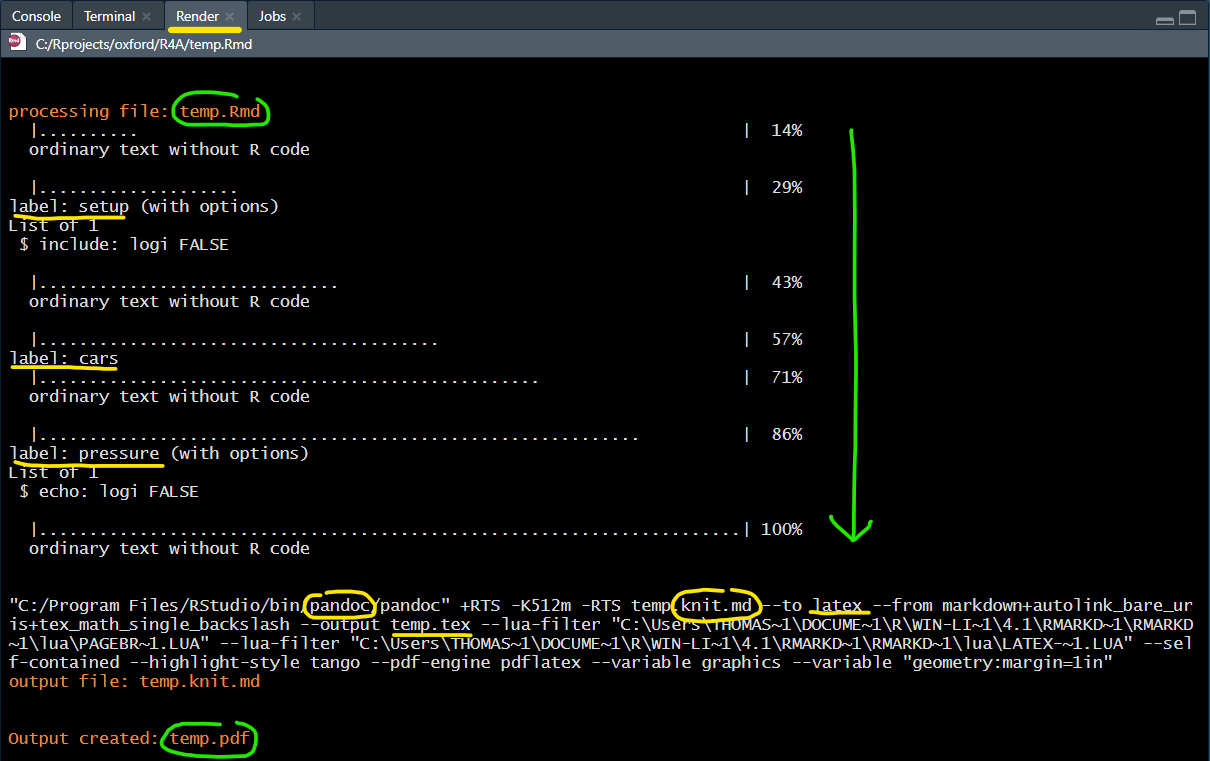
\includegraphics[width=7.29167in,height=\textheight]{www/rmd_render.png}

\hypertarget{publishing-on-platforms}{%
\section{Publishing on platforms}\label{publishing-on-platforms}}

\hypertarget{references}{%
\section{References}\label{references}}

\end{document}
